\documentclass[dissertation.tex]{subfiles}
\begin{document}

\chapter{Large-scale subjective evaluation}

\cite{pearce2001towards} addresses difficulty in quantitative evaluation,
suggesting the use of a learned critic in a manner similar to GANs
\cite{goodfellow2014generative}. In a later report,
\cite{pearce2002motivations} attribute difficulty in evaluation due to lack
aim: algorithmic composition, design of compositional tools, and computational
modelling of musical styles or music cognition all have different motivations
and should thus be evaluated differently.

Following advice of \cite{pearce2002motivations}, we identify our key
motivation as algorithmic composition: generation of novel compositions.
To evaluate our success, we employ a subjective evaluation method.

\cite{ariza2009} criticizes a musical Turing test as providing little data about
how to improve the system, suggesting that listener studies using music experts
may be more insightful.

The frontend utilizes React and Redux, allowing us to collect fine-grained user
action data. Azure App Service is used to host an Express web-service which
randomizes experimental questions and collects responses. The data is stored to
Azure Data Storage and processed in batch MapReduce using Azure HDInsight.

\begin{figure}[htpb]
  \centering
  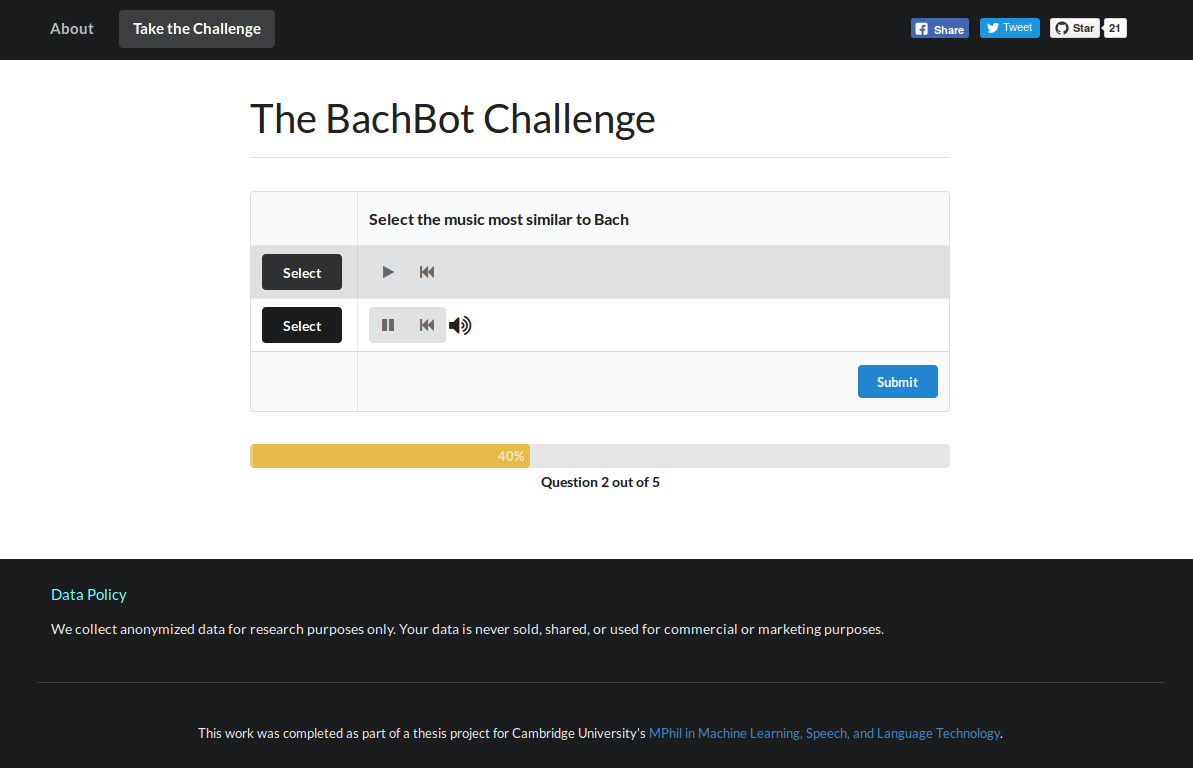
\includegraphics[width=1.0\linewidth]{Figures/question-screen.png}
  \caption{Figures/question-Screen}
  \label{fig:Figures/question-screen}
\end{figure}

\begin{figure}[htpb]
  \centering
  
\includegraphics[width=1.0\linewidth]{Figures/user-info-form.png}
  \caption{Figures/}
  \label{fig:user-info-form}
\end{figure}

We ask users to rate themselves on their musical skills (0-10) and present the
user with five questions. Each questions asks the user to listen to two
samples, one generated and one original Bach, and tasks the user to select the
original. In addition to the question response, we collect data on the time
spent on a questions and number of times each sample is played.

\section{Results}

\subsection{Participant backgrounds and demographics}

\begin{figure}[htpb]
  \centering
  \begin{subfigure}[b]{0.98\textwidth}
    \centering
    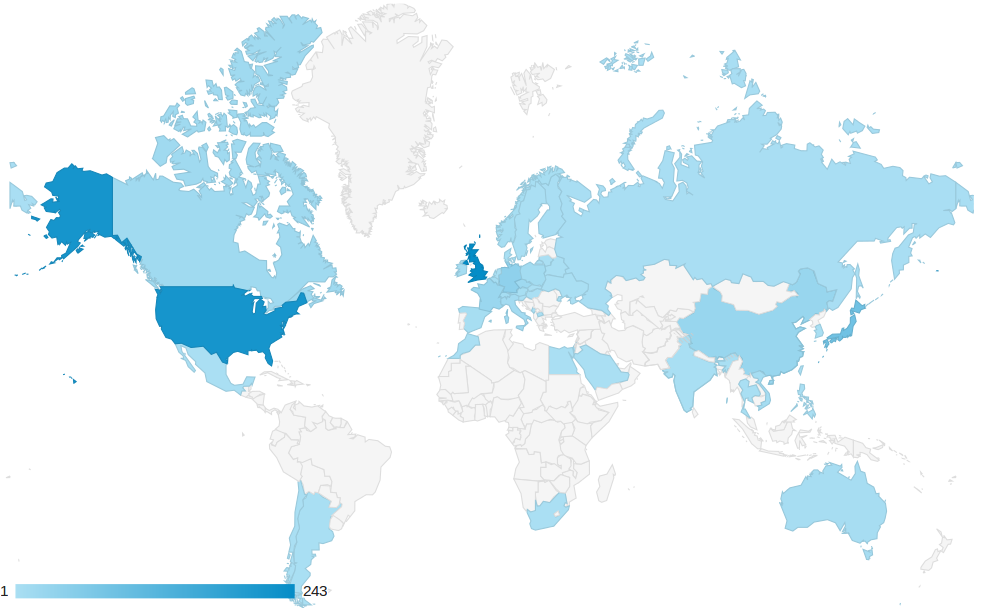
\includegraphics[width=1.0\linewidth]{Figures/participants-by-country.png}
  \end{subfigure}
  \begin{subfigure}[b]{0.48\textwidth}
    \centering
    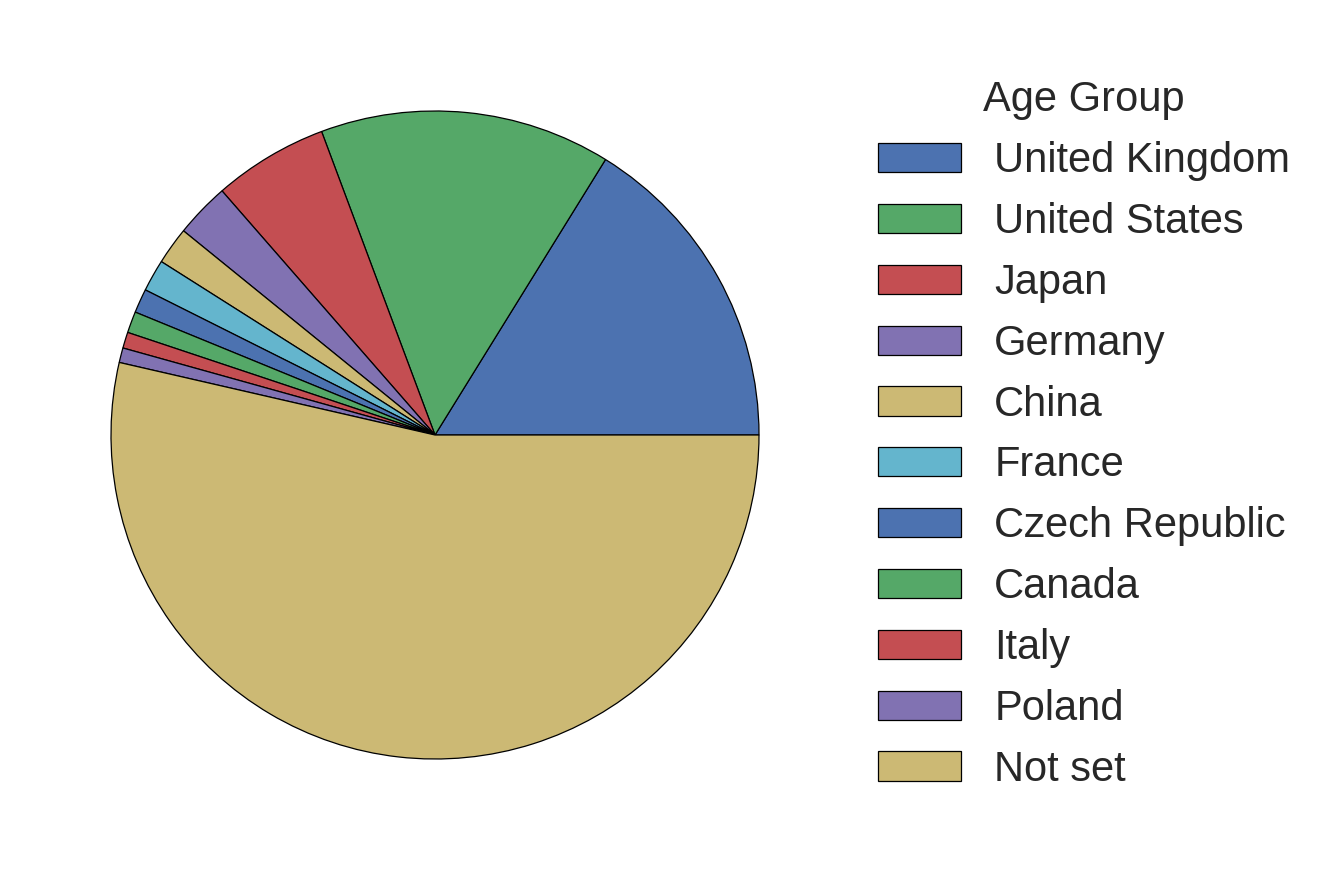
\includegraphics[width=1.0\linewidth]{Figures/user-demographics-pie.png}
  \end{subfigure}
  \begin{subfigure}[b]{0.48\textwidth}
    \centering
    \begin{tabular}{lrr}
\toprule
Country        &  Responses       &  Proportion \\
\midrule
UK             &       243 &            16.0\% \\
US             &       218 &            15.0\% \\
Japan          &        86 &             6.0\% \\
Germany        &        41 &             3.0\% \\
China          &        28 &             2.0\% \\
France         &        24 &             2.0\% \\
Czechia        &        18 &             1.0\% \\
Canada         &        16 &             1.0\% \\
Italy          &        12 &             1.0\% \\
Poland         &        11 &             1.0\% \\
Not set        &       805 &            54.0\% \\
\bottomrule
\end{tabular}

  \end{subfigure}
  \caption{Figures/user-demographics-Pie}
  \label{fig:Figures/user-demographics-pie}
\end{figure}

\begin{figure}[htpb]
  \centering
  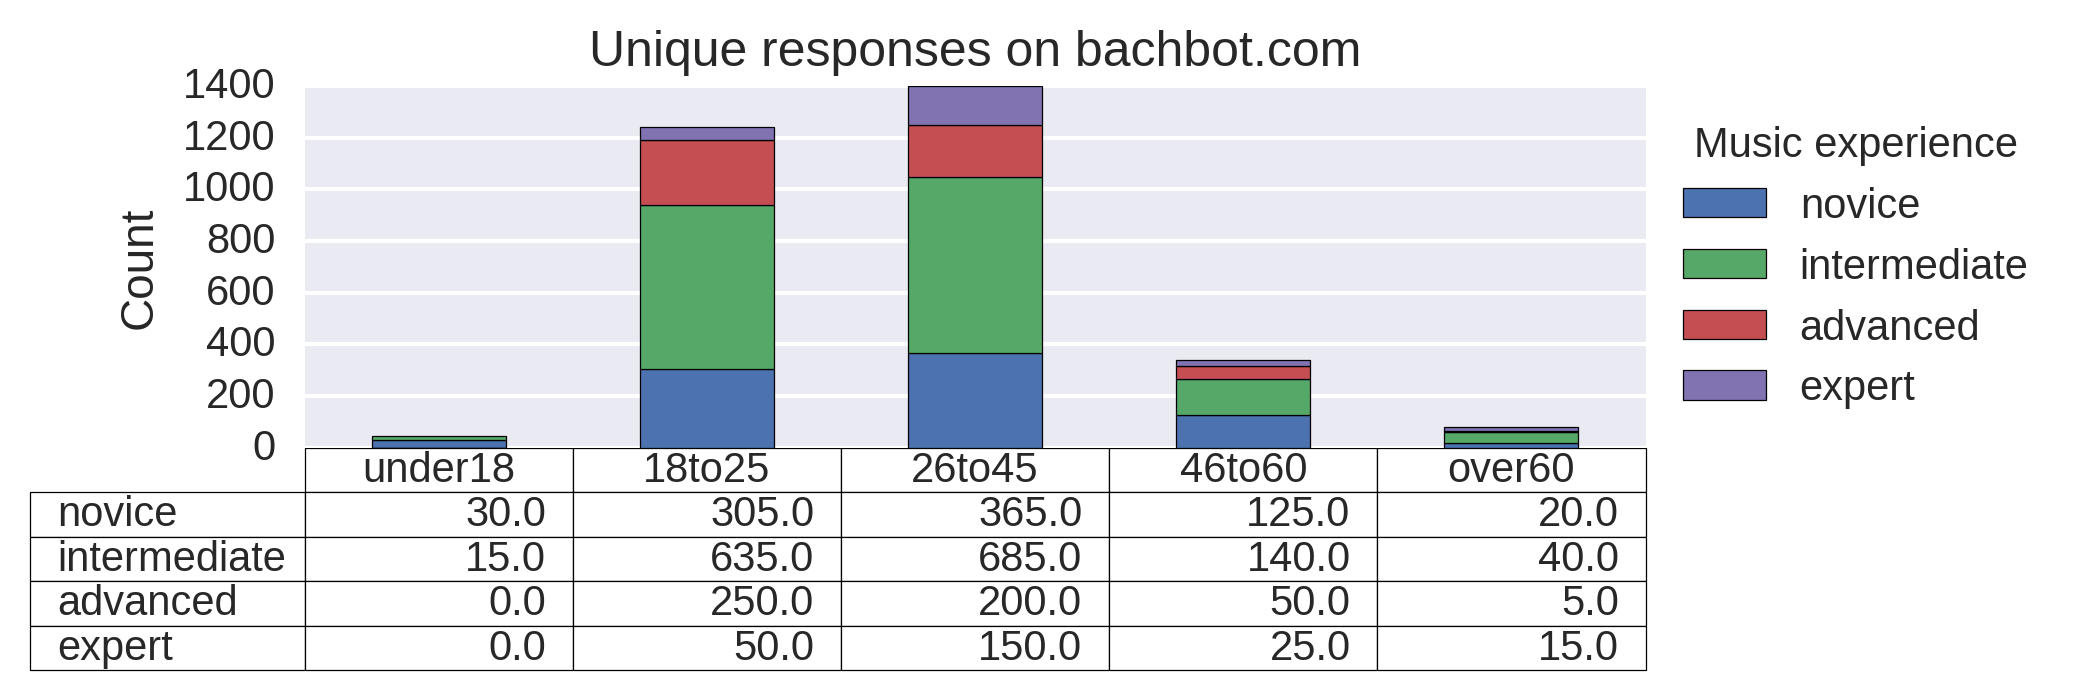
\includegraphics[width=1.0\linewidth]{Figures/responses-ageGroup-musicExperience.png}
  \caption{Demographic breakdown of participants}
  \label{fig:responses-ageGroup-musicExperience}
\end{figure}

\todo{\autoref{fig:responses-mask} suggests performance is weakest on
  harmonizations. Unsurprising because we only do 1-best and don't account
  for future. Bidirectional LSTM or N-best lattice search (reference marcin)
  would do better}
\begin{figure}[htpb]
  \centering
  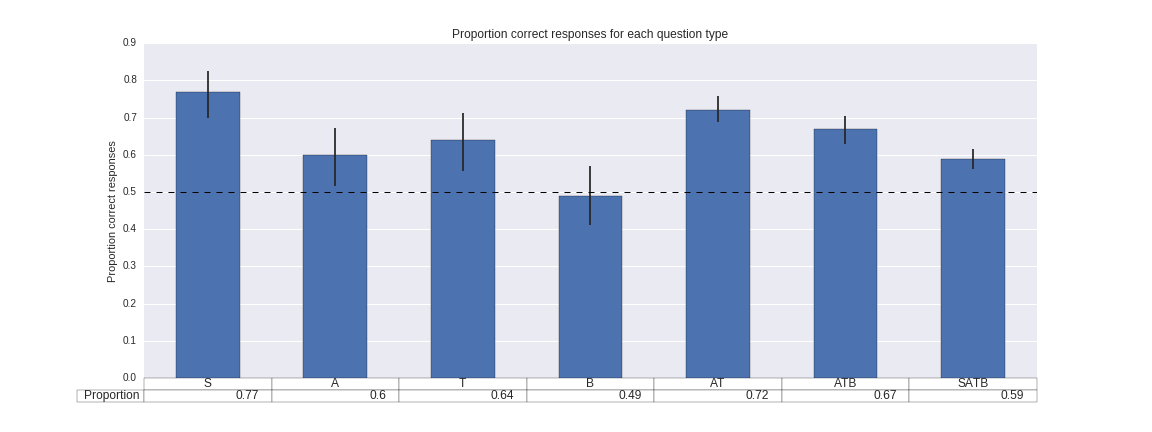
\includegraphics[width=1.0\linewidth]{Figures/responses-mask.png}
  \caption{Figures/responses-Mask}
  \label{fig:responses-mask}
\end{figure}

\begin{figure}[htpb]
  \centering
  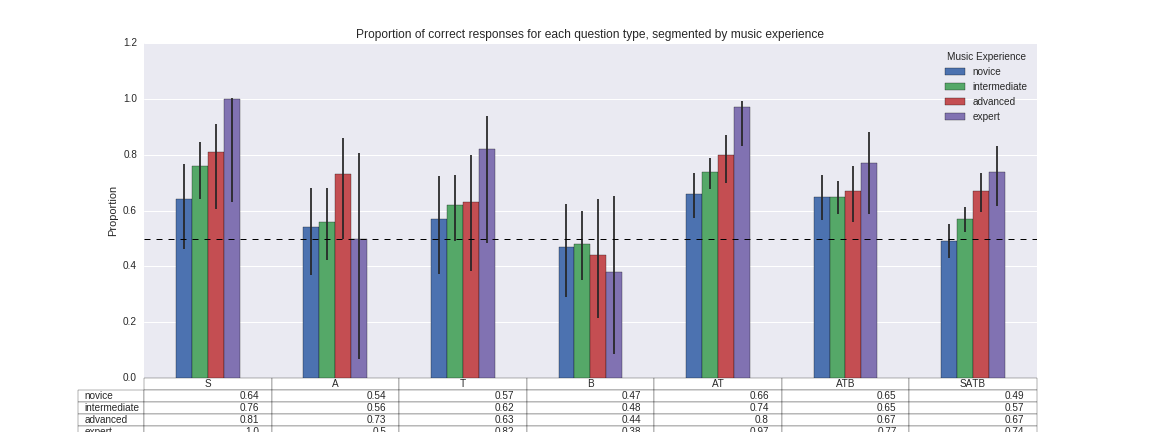
\includegraphics[width=1.0\linewidth]{Figures/responses-mask-musicExperience.png}
  \caption{Figures/responses-mask-MusicExperience}
  \label{fig:responses-mask-musicExperience}
\end{figure}

\begin{figure}[htpb]
  \centering
  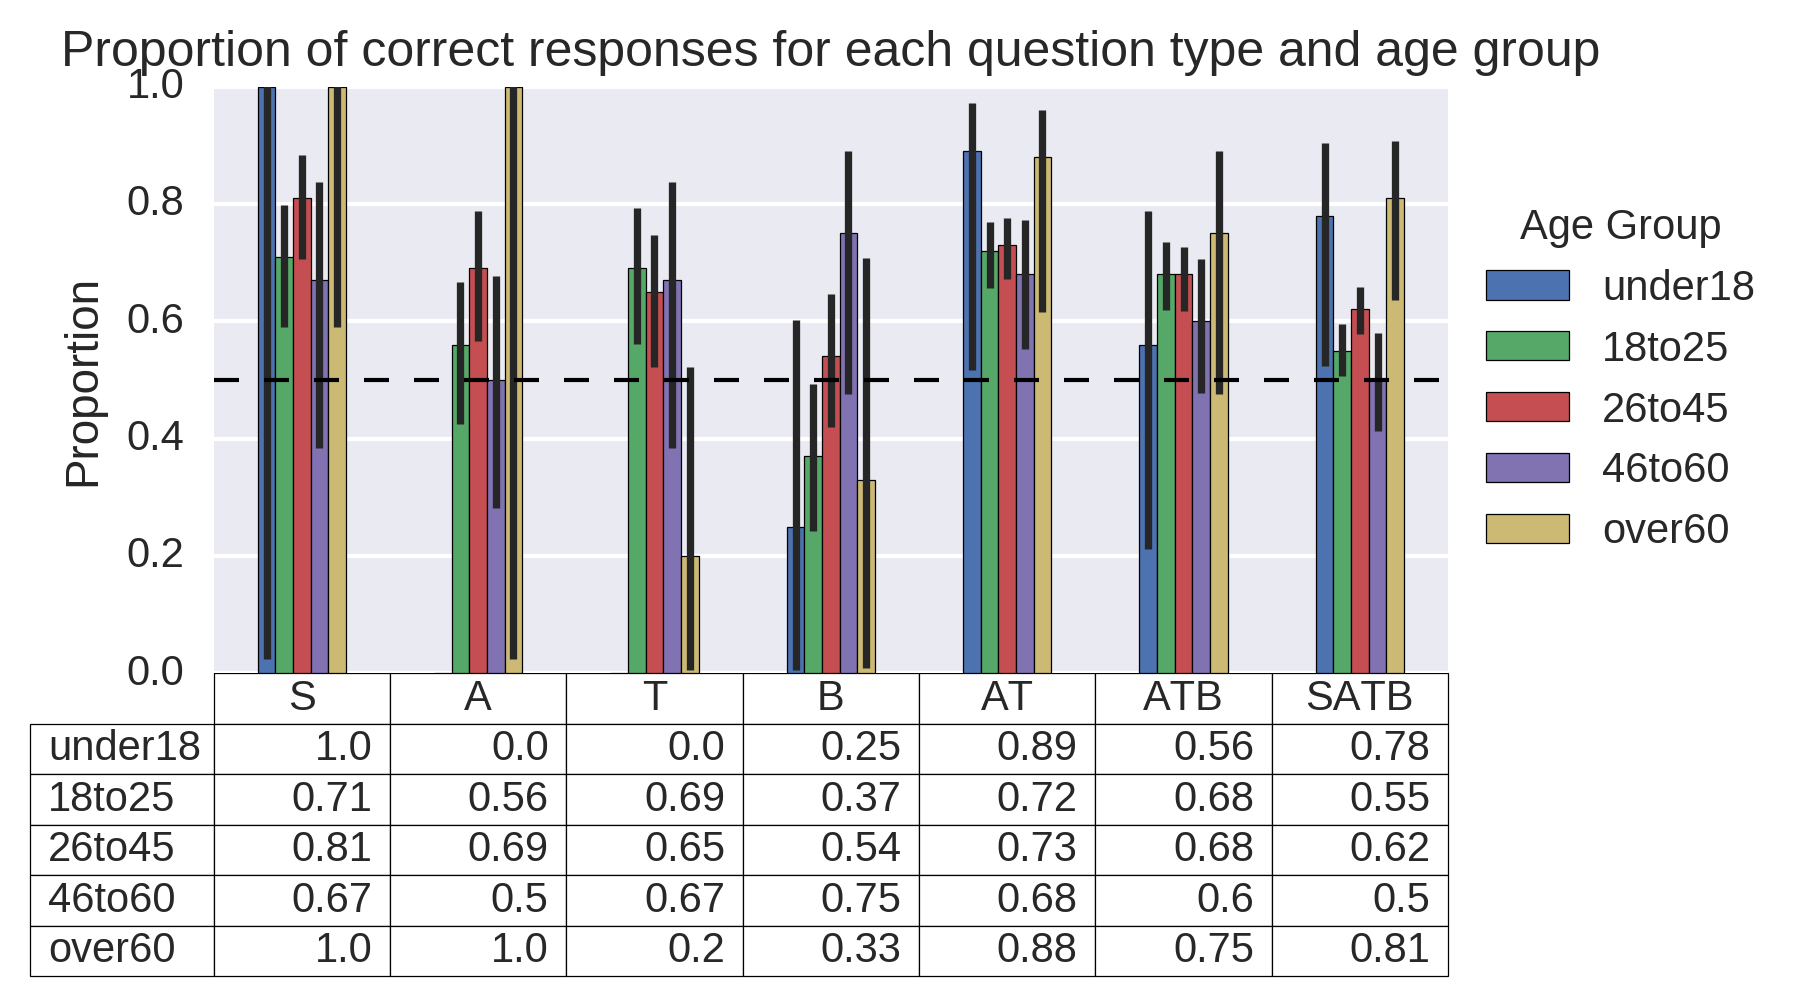
\includegraphics[width=1.0\linewidth]{Figures/responses-mask-agegroup.png}
  \caption{Figures/responses-mask-Agegroup}
  \label{fig:responses-mask-agegroup}
\end{figure}

\begin{figure}[htpb]
  \centering
  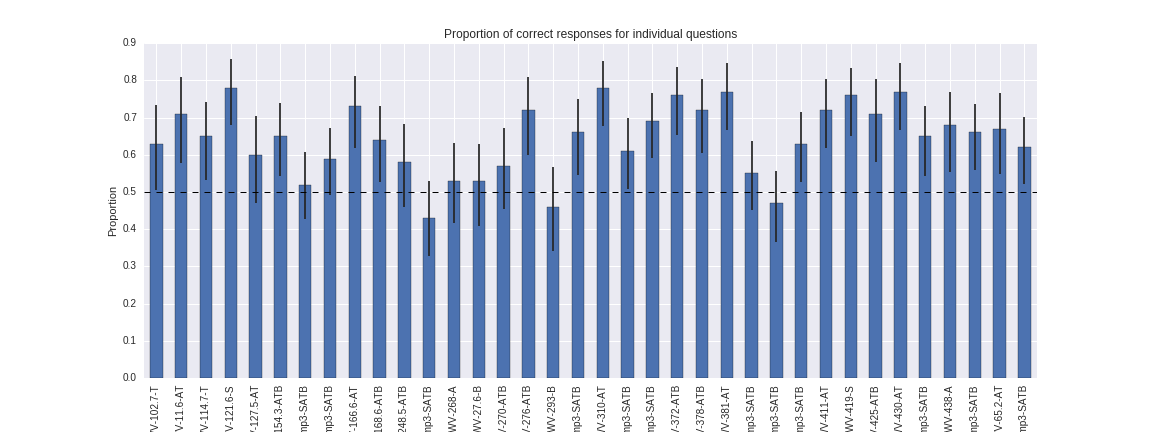
\includegraphics[width=1.0\linewidth]{Figures/responses-name.png}
  \caption{Proportion of correct responses broken down by individual questions.}
  \label{fig:responses-name}
\end{figure}

\todo{Analyze why bad questions in \autoref{fig:responses-name} are happening}

\section{User feedback}

The modulations and part writing were the giveaway for me (and once or twice the phrasing)

Got 5/5. The trick is to listen for the unnatural pauses at regular intervals.

Cool project, I scored 100\% so I'm quite pleased with myself ;o) I do
play an instrument although I'm not classical trained. If I had an
inkling to why I could choose the background phrasing of the Bach
pieces is far more elegant than the computer generated pieces.

@samim @feynmanliang really impressive! If I didn't know about counterpoint that quiz would've stumped me



\printbibliography

\end{document}
